%!TEX root = ../../thesis.tex

\section{Experiments}
\label{sec:sar-experiments}

\subsection{Datasets}

We evaluate our model on \sys{CNN/Daily Mail}~\cite{hermann2015teaching} and \sys{SQuAD}~\cite{rajpurkar2016squad}, the two most popular and competitive reading comprehension datasets. We have described them before in Section~\ref{sec:deep-learning-era} regarding their importance in the development of neural reading comprehension and the way the datasets were constructed. Now we give a brief review of these datasets and the statistics.

\begin{itemize}
\item
The \sys{CNN/Daily Mail} datasets were made from articles on the news websites CNN and Daily Mail, utilizing articles and their bullet point summaries. One bullet point is converted to a question with one entity replaced by a placeholder and the answer is this entity. The text has been run through a Google NLP pipeline. It it tokenized, lowercased, and named entity recognition and coreference resolution have been run. For each coreference chain containing at least one named entity, all items in the chain are replaced by an @entity$n$ marker, for a distinct index $n$ (Table~\ref{tab:rc-examples} (a)). On average, both the \sys{CNN} and \sys{Daily Mail} contain 26.2 different entities in the article. The training, development, and testing examples were collected from the news articles at different times. The accuracy (percentage of examples predicting the correct entity) is used for evaluation.

\item
The \sys{SQuAD} dataset was collected based on Wikipedia articles. 536 high-quality Wikipedia articles were sampled and crowdworkers created questions based on each individual paragraph (paragraphs shorter than 500 characters were discarded), requiring that answer must be highlighted from the paragraph (Table~\ref{tab:rc-examples} (c)). The training/development/testing splits were made randomly based on articles (80\% vs. 10\% vs. 10\%). To estimate human performance and also make evaluation more reliable, they collected a few additional answers for each question (each question in the development set has 3.3 answers on average). Exact match and macro-averaged F1 scores are used for evaluation, as we discussed in Section~\ref{sec:evaluation}. Note that \sys{SQuAD} 2.0~\cite{rajpurkar2018know} was proposed more recently, which added 53,775 unanswerable questions to the original dataset and we will discuss it in Section~\ref{sec:future-datasets}. For most of this thesis, \sys{SQuAD} refers to \sys{SQuAD} 1.1 unless stated otherwise.
\end{itemize}


\begin{table}[t]
  \centering
  \begin{tabular}{l | r r | r }
  \hline
    & \multicolumn{2}{c|}{cloze style} & span prediction \\
    & \tf{CNN} & \tf{Daily Mail} & \tf{SQuAD} \\
  \hline
  \#Train & 380,298 & 879,450 & 87,599 \\
  \#Dev & 3,924 & 64,835 & 10,570 \\
  \#Test & 3,198 & 53,182 & 9,533 \\
  \hline
  Passage: avg. tokens & 761.8 & 813.1 & 134.4 \\
  Question: avg. tokens & 12.5 & 14.3 & 11.3 \\
  Answer: avg. tokens & 1.0 & 1.0 & 3.1 \\
  \hline
  \end{tabular}
  \longcaption{Data statistics of \sys{CNN/Daiily Mail} and \sys{SQuAD}}{\label{tab:data-statistics}Data statistics of \sys{CNN/Daily Mail} and \sys{SQuAD}. The average numbers of tokens are computed based on the training set.}
\end{table}


Table~\ref{tab:data-statistics} gives more detailed statistics of the datasets. As it is shown, the \sys{CNN/Daily Mail} datasets are much larger than \sys{SQuAD} (almost one order of magnitude bigger) due to the way the datasets were constructed. The passages used in \sys{CNN/Daily Mail} are also much longer --- 761.8 and 813.1 tokens for \sys{CNN} and \sys{Daily Mail} respectively, while it is 134.4 tokens for SQuAD. Finally, the answers in \sys{SQuAD} consists of only 3.1 tokens on average, which reflects the fact the most of the \sys{SQuAD} questions are factoid and a large portion of the answers are common nouns or named entities.


\subsection{Implementation Details}
\label{sec:imp-details}

Besides different model architecture designs, implementation details also play a crucial role in the final performance of these neural reading comprehension systems. In the following we highlight a few important aspects that we haven't covered yet and finally give the model specifications that we used on the two datasets.

\paragraph{Stacked BiLSTMs.} One simple idea is to increase the depth of bidirectional LSTMs for question and passage encoding. It computes $\mf{h}_t = [\overrightarrow{\mf{h}}_t; \overleftarrow{\mf{h}}_t] \in \R^{2h}$ and then regard $\mf{h}_t$ as the input $\mf{x}_t$ of the next layer and pass them into another BiLSTM, and so on. We generally find that stacking BiLSTMs works better than a one-layer BiLSTM and we used $3$ layers for the SQuAD experiment.\footnote{We only used a shallow one-layer BiLSTM for the CNN/Daily Mail experiments in 2016 though.}

\paragraph{Dropout.} Dropout is an effective and widely used approach to regularization in neural networks. Simply put, dropout refers to masking out some units at random during the training process. For our model, dropout can be added to the word embeddings, input vectors and hidden vectors of every LSTM layer. Finally, the variational dropout approach \cite{gal2016theoretically} has demonstrated to work better than the standard dropout on regularizing RNNs. The idea is to apply the same dropout mask at each time step for both inputs, outputs and recurrent layers, i.e., the same units are dropped at each time step. We suggest readers to use this variant in practice.\footnote{We didn't include variational dropout in our published paper results but later found it useful.}

\paragraph{Handling word embeddings.} One common way (and also our default choice) to handle word embeddings is to keep the most frequent $K$ (e.g., $K = 500,000$) word types in the training set and map all other words to an $\left<unk\right>$ token and then use pre-trained word embeddings to initialize the $K$ words. Typically, when the training set is large enough, we fine tune all the word embeddings; when the training set is relatively small (e.g., \sys{SQuAD}), we usually keep all the word embeddings fixed as static features. In \newcite{chen2017reading}, we find that it helps to fine-tune the most frequent question words because the representations of these key words such as \ti{what}, \ti{how}, \ti{which} could be crucial for reading comprehension systems. Some studies such as \cite{dhingra2017comparative} demonstrated the use of pre-trained embeddings and the ways of handling out-of-vocabulary words have a large impact on the performance of reading comprehension tasks.

\paragraph{Model specifications.}
For all the experiments which require linguistic annotations (lemma, part-of-speech tags, named entity tags, dependency parses), we use the Stanford CoreNLP toolkit~\cite{manning2014stanford} for preprocessing. For training all the neural models, we sort all the examples by the length of its passage, and randomly sample a mini-batch of size 32 for each update.

For the results on \sys{CNN/Daily Mail}, we use the lowercased, 100-dimensional pre-trained \sys{Glove} word embeddings~\cite{pennington2014glove} trained on Wikipedia and Gigaword for initialization. The attention and output parameters are initialized from a uniform distribution between $(-0.01, 0.01)$, and the LSTM weights are initialized from a Gaussian distribution $\mathcal{N}(0, 0.1)$. We use a 1-layer BiLSTM of hidden size $h = 128$ for \sys{CNN} and $h = 256$ for \sys{Daily Mail}. Optimization is carried out using vanilla stochastic gradient descent (SGD), with a fixed learning rate of $0.1$.  We also apply dropout with probability $0.2$ to the embedding layer and gradient clipping when the norm of gradients exceeds $10$.

For the results on \sys{SQuAD}, we use 3-layer BiLSTMs with $h = 128$ hidden units for both paragraph and question encoding. We use \sys{Adamax} for optimization as described in \cite{kingma2014adam}. Dropout with probably $0.3$ is applied to word embeddings and all the hidden units of LSTMs. We used the $300$-dimensional \sys{Glove} word embeddings trained from 840B Web crawl data for initialization and only fine-tune the 1000 most frequent question words.

Other implementation details can be found in the following two Github repositories:
\begin{itemize}
    \item
        \href{https://github.com/danqi/rc-cnn-dailymail}{https://github.com/danqi/rc-cnn-dailymail} for our experiments in \newcite{chen2016thorough}.
    \item
        \href{https://github.com/facebookresearch/DrQA}{https://github.com/facebookresearch/DrQA} for our experiments in \newcite{chen2017reading}.
\end{itemize}

We also would like to caution readers that our experimental results were published in two papers (2016 and 2017) and they differ in various places. A key difference is that our results on \sys{CNN/Daily Mail} didn't include manual features $f_{token}(p_i)$, exact match features $f_{exact\_match}(p_i)$, aligned question embeddings $f_{align}(p_i)$ and $\tilde{\mf{p}}_i$ just takes the word embedding $\mf{E}(p_i)$. Another difference is that we didn't have the attention layer in question encoding before but simply concatenated the last hidden vectors from the LSTMs in both directions. We believe that that these additions are useful on \sys{CNN/Daily Mail} and other cloze style tasks as well, but we didn't further investigate it.


\subsection{Experimental Results}

\subsubsection{Results on \sys{CNN/Daily Mail}}

\begin{table}[t]
\centering
\begin{tabular}{l c c c c}
\toprule
\multirow{2}{*}{\tf{Model}} & \multicolumn{2}{c}{\sys{CNN}} &  \multicolumn{2}{c}{\sys{Daily Mail}} \\
& \tf{Dev} & \tf{Test} & \tf{Dev} & \tf{Test} \\
\midrule
 Frame-semantic model $^\dagger$ &36.3  & 40.2 & 35.5 & 35.5 \\
 Word distance model $^\dagger$ & 50.5 & 50.9 & 56.4 & 55.5 \\
 Deep LSTM Reader $^\dagger$ & 55.0 & 57.0 & 63.3 & 62.2 \\
Attentive Reader $^\dagger$ & 61.6 & 63.0 & 70.5 & 69.0 \\
 Impatient Reader $^\dagger$ & 61.8 & 63.8 & 69.0 & 68.0 \\
\midrule
MemNNs (window memory) $^\ddagger$ & 58.0 & 60.6 & N/A & N/A \\
MemNNs (window memory + self-sup.) $^\ddagger$ & 63.4 & 66.8 & N/A & N/A\\
MemNNs (ensemble) $^\ddagger$ & 66.2\rlap{$^*$} & 69.4\rlap{$^*$} & N/A & N/A \\
\midrule
Our feature-based classifier & 67.1 & 67.9 & 69.1 & 68.3 \\
\midrule
Stanford Attentive Reader & 72.5 & 72.7 & 76.9 & 76.0 \\
Stanford Attentive Reader (ensemble) &  76.2\rlap{$^*$} & 76.5\rlap{$^*$} & 79.5\rlap{$^*$} & 78.7\rlap{$^*$} \\
\bottomrule
\end{tabular}
\longcaption{Evaluation results on CNN/Daily Mail}{\label{tab:cnn-dm-results}Accuracy of all models on the \sys{CNN} and \sys{Daily Mail} datasets. Results marked $^\dagger$ are from \newcite{hermann2015teaching} and results marked $^\ddagger$ are from \newcite{hill2016goldilocks}. The numbers marked with $^*$ indicate that the results are from ensemble models.}
\end{table}


Table~\ref{tab:cnn-dm-results} presents the results that we reported in \newcite{chen2016thorough}. We run our neural models 5 times independently with different random seeds and report average performance across the runs. We also report ensemble results which average the prediction probabilities of the 5 models. We also present the results for the feature-based classifier we described in Section~\ref{sec:feature-models}.

\paragraph{Baselines.} We were among the earliest groups to study this first large-scale reading comprehension dataset. At the time, \newcite{hermann2015teaching} and \newcite{hill2016goldilocks} proposed a few baselines, both symbolic approaches and neural models, for this task. The baselines include:
\begin{itemize}
    \item
        A \sys{frame-semantic} model in \newcite{hermann2015teaching}, which they run a state-of-the-art semantic parser, and extract entity-predicate triples denoted as $(e_1, V, e_2)$ from both the question and the passage, and attempt to match the correct entity using a number of heuristic rules.
    \item
        A \sys{word distance} model in \newcite{hermann2015teaching}, in which they align the placeholder of the question with each possible entity, and compute a distance measure between the question and the passage around the aligned entity.
    \item
        Several LSTM-based neural models proposed in \newcite{hermann2015teaching}, named \sys{Deep LSTM Reader}, \sys{Attentive Reader} and \sys{Impatient Reader}. The \sys{Deep LSTM Reader} just processes the question and the passage as one sequence using a deep LSTM (without attention mechanism), and makes a prediction in the end. The \sys{Attentive Reader} is similar in spirit to ours, as it computes an attention function between the question vector and all the passage vectors; while the \sys{Impatient Reader} computes an attention function for all the question words and recurrently accumulates information as the model reads each question word.
    \item
        \sys{Window-based memory networks} proposed by \newcite{hill2016goldilocks} is based on the memory network architecture \cite{weston2015memory}. We think the model is also similar to ours and the biggest difference is their way of encoding passages: they only use a 5-word context window when evaluating a candidate entity and they use a positional unigram approach to encode the contextual embeddings. If a window consists of $5$ words $x_1, x_2, \ldots, x_5$, then it is encoded as $\sum{\mf{E}_i(x_i)}$, resulting in $5$ separate embedding matrices to learn. They encode the $5$-word window surrounding the placeholder in a similar way and all other words in the question text are ignored. In addition, they simply use a dot product to compute the ``relevance'' between the question and a contextual embedding.
\end{itemize}

As seen in Table~\ref{tab:cnn-dm-results}, our feature-based classifier obtains 67.9\% accuracy on the \sys{CNN} test set and 68.3\% accuracy on the \sys{Daily Mail} test set. It significantly outperforms any of the symbolic approaches reported in \newcite{hermann2015teaching}. We feel that their frame-semantic model is not suitable for these tasks due to the poor coverage of the parser and is not representative of what a straightforward NLP system can achieve. Indeed, the frame-semantic model is even markedly inferior to the word distance model. To our surprise, our feature-based classifier even outperforms all the neural network systems in \newcite{hermann2015teaching} and the best single-system result reported from \newcite{hill2016goldilocks}.   Moreover, our single-model neural network surpasses the previous results by a large margin (over 5\%), pushing up the state-of-the-art accuracies to 72.7\% and 76.0\% respectively. The ensembles of 5 models consistently bring further 2-4\% gains.

\subsubsection{Results on \sys{SQuAD}}
\begin{table}[t]
\begin{center}
\begin{tabular}{p{8.5cm} c c c c}
\hline
 \bf Method &  \multicolumn{2}{c}{\bf Dev} & \multicolumn{2}{c}{\bf Test} \\
&  \tf{EM} & \tf{F1} & \tf{EM} & \tf{F1} \\
\hline
Logistic regression \cite{rajpurkar2016squad} & 40.0 & 51.0 & 40.4 & 51.0 \\
\hline
Match-LSTM~\cite{wang2017machine} &  64.1 & 73.9 & 64.7 & 73.7 \\
RaSoR~\cite{lee2016learning} & 66.4 & 74.9 & 67.4 & 75.5 \\
DCN~\cite{xiong2017dynamic} & 65.4 & 75.6 & 66.2 & 75.9 \\
BiDAF~\cite{seo2017bidirectional}  & 67.7 & 77.3 & 68.0 & 77.3 \\
\hline
\tf{Our model}~\cite{chen2017reading} & 69.5 & 78.8 & 70.0 &  79.0\\
\hline
R-NET~\cite{wang2017gated} & 71.1 & 79.5 & 71.3 & 79.7 \\
BiDAF + self-attention~\cite{peters2018deep} & N/A & N/A & 72.1 & 81.1 \\
FusionNet~\cite{huang2018fusionnet} & N/A & N/A & 76.0 & 83.9 \\
QANet~\cite{yu2018qanet} & 73.6 & 82.7 & N/A & N/A \\
SAN~\cite{liu2018stochastic} & 76.2 & 84.1 & 76.8 & 84.4 \\
{\small BiDAF + self-attention + ELMo}~\cite{peters2018deep} & N/A & N/A & 78.6 & 85.8 \\
BERT~\cite{devlin2018bert} & 84.1 & 90.9 & N/A & N/A \\
\hline
Human performance \cite{rajpurkar2016squad} & 80.3 & 90.5 & 82.3 & 91.2 \\
\hline
\end{tabular}
\end{center}
\longcaption{Evaluation results on SQuAD}{\label{tab:squad-results} Evaluation results on the SQuAD dataset (single model only). The results below ``our model'' were released after we finished the paper in Feb 2017. We only list representative models and report the results from the published papers. For a fair comparison, we didn't include the results which use other training resources (e.g., TriviaQA) or data augmentation techniques, except pre-trained language models, but we will discuss them in Section~\ref{sec:advances}. }
\end{table}

Table~\ref{tab:squad-results} presents our evaluation results on both the development and testing sets. SQuAD has been a very competitive benchmark since it was created and we only list a few representative models and the single-model performance. It is well known that the ensemble models can further improve the performance by a few points. We also included results from the logistic regression baseline (i.e., feature-based classifiers) created by the original authors \cite{rajpurkar2016squad}.


Our system can achieve 70.0\% exact match and 79.0\% F1 scores on the test set, which surpassed all the published results and matched the top performance on the SQuAD leaderboard\footnote{\href{https://stanford-qa.com}{https://stanford-qa.com}.} at the time we wrote the paper~\cite{chen2017reading}. Additionally, we think that our model is conceptually simpler than most of the existing systems. Compared to the logistic regression baseline, which gets $\text{F1} = 51.0$, this model is already close to a 30\% absolute improvement and it is a big win for neural models.

Since then, \sys{SQuAD} has received tremendous attention and great progress has been made on this dataset, as seen in Table~\ref{tab:squad-results}. Recent advances include pre-trained language models for initialization, more fine-grained attention mechanisms, data augmentation techniques and even better training objectives. We will discuss them in Section~\ref{sec:advances}.


\subsubsection{Ablation studies}

\begin{table}[h]
	\begin{center}
	\begin{tabular}{l | l}
    \hline
    \bf Features & \bf F1\\
    \hline
    Full & 78.8 \\
    \hline
    No $f_{token}$ & 78.0 (-0.8)\\
    No $f_{exact\_match}$ & 77.3 (-1.5)\\
    No $f_{aligned}$ & 77.3 (-1.5)\\
    No $f_{aligned}$ and $f_{exact\_match}$ & 59.4 (-19.4) \\
    \hline
    \end{tabular}
    \end{center}
    \longcaption{Feature ablation analysis on SQuAD}{\label{tab:feature-ablation}Feature ablation analysis of the paragraph representations of our model. Results are reported on the SQuAD development set.}
\end{table}

In \newcite{chen2017reading}, we conducted an ablation analysis on the components of the passage representations. As shown in Table~\ref{tab:feature-ablation}, all the components contribute to the performance of our final system. We find that, without the aligned question embeddings (only word embeddings and a few manual features), our system is still able to achieve F1 over ~77\%. The effectiveness of exact match features $f_{exact\_match}$ also indicates that there are a lot of words overlapping between the passage and the question on this dataset. More interestingly, if we remove both $f_{aligned}$ and $f_{exact\_match}$, the performance drops dramatically, so we conclude that both features play a similar but complementary role in the feature representation, like the hard and soft alignments between question and passage words.

% \subsubsection{Attention visualization}
% \red{TODO}


\subsection{Analysis: What Have the Models Learned?}

In \newcite{chen2016thorough}, we attempted to understand better what these models have actually learned, and what depth of language understanding is needed to solve these problems. We approach this by doing a careful hand-analysis of 100 randomly sampled examples from the development set of the \sys{CNN} dataset.

We roughly classify them into the following categories (if an example satisfies more than one category, we classify it into the earliest one):
\begin{description}
   \item[\tf{Exact match}] The nearest words around the placeholder are also found in the passage surrounding an entity marker; the answer is self-evident.
   \item[\tf{Sentence-level paraphrasing}] The question text is entailed\slash rephrased by \ti{exactly} one sentence in the passage, so the answer can definitely be identified from that sentence.
   \item[\tf{Partial clue}] In many cases, even though we cannot find a complete semantic match between the question text and some sentence, we are still able to infer the answer through partial clues, such as some word/concept overlap.
   \item[\tf{Multiple sentences}] Multiple sentences must be processed to infer the correct answer.
   \item[\tf{Coreference errors}] It is unavoidable that there are many coreference errors in the dataset. This category includes those examples with critical coreference errors for the answer entity or key entities appearing in the question. Basically we treat this category as ``not answerable''.
   \item[\tf{Ambiguous or hard}] This category includes examples for which we think humans are not able to obtain the correct answer (confidently).
\end{description}

Table~\ref{tab:cnn-ex-breakdown} provides our estimate of the percentage for each category, and Figure~\ref{fig:cnn-examples} presents one representative example from each category. We observe that \ti{paraphrasing} accounts for 41\% of the examples and 19\% of the examples are in the \ti{partial clue} category. Adding the most simple \ti{exact match} category, we hypothesize a large portion (73\% in this subset) of the examples are able to be answered by identifying the most relevant (single) sentence and inferring the answer based upon it. Additionally, only 2 examples require multiple sentences for inference. This is a lower rate than we expected and this suggests that the dataset requires less reasoning than previously thought. To our surprise, “coreference errors” and “ambiguous/hard” cases account for 25\% of this sample set, based on our manual analysis, and this certainly will be a barrier for training models with an accuracy much above 75\% (although, of course, a model can sometimes make a lucky guess). In fact, our ensemble neural network model is already able to achieve 76.5\% on the development set, and we think that the prospect for further improving on this dataset is small.

\begin{figure}[p]
\centering
\begin{tabular}{l p{4.5cm} p{6.5cm}}
\toprule
Category & Question & Passage \\
\midrule
Exact Match & \ti{it 's clear @entity0 is leaning toward} {\tf{@placeholder}} ,  says an expert who monitors @entity0 & \ldots @entity116 , who follows @entity0 's operations and propaganda closely , recently told @entity3 , \ti{it 's clear @entity0 is leaning toward} \tf{@entity60}  in terms of doctrine , ideology and an emphasis on holding territory after operations . \ldots  \\
\midrule
Paraphrasing & {\tf{@placeholder} says he understands why @entity0 wo n't play at his tournament} &  \ldots @entity0 called me personally to let me know that he would n't be playing here at @entity23 , " \tf{@entity3} said on his @entity21 event 's website . \ldots \\
\midrule
Partial clue & a tv movie based on @entity2 's book \tf{@placeholder} casts a @entity76 actor as @entity5 & \ldots  to @entity12  @entity2 professed that his \tf{@entity11} is not a religious book . \ldots \\
\midrule
Multiple sent. &  he 's doing a his - and - her duet all by himself ,  @entity6 said of \tf{@placeholder} &  \ldots we got some groundbreaking performances , here too , tonight ,  @entity6 said . we got \tf{@entity17} , who will be doing some musical performances . he 's doing a his - and - her duet all by himself .  \ldots \\
\midrule
Coref. Error & rapper \tf{@placeholder} " disgusted , " cancels upcoming show for @entity280 & \ldots with hip - hop star \tf{@entity246} saying on @entity247 that he was canceling an upcoming show for the @entity249 . \ldots  (but @entity249 = @entity280 = SAEs)\\
\midrule
Hard & pilot error and snow were reasons stated for \tf{@placeholder} plane crash  & \ldots a small aircraft carrying \tf{@entity5} , @entity6 and @entity7 the @entity12  @entity3 crashed a few miles from @entity9 , near @entity10 , @entity11 . \ldots \\
\bottomrule
\end{tabular}
\longcaption{Some representative examples from each category}{\label{fig:cnn-examples}Some representative examples from each category on the \sys{CNN} dataset.}
\end{figure}

\begin{table}[!t]
  \centering
    \begin{tabular}{l  l  r}
      \toprule
    \tf{\#} & \tf{Category} &    \\
    \midrule
    1 & Exact match & 13\%   \\
    2 & Paraphrasing & 41\% \\
    3 & Partial clue & 19\%  \\
    4 & Multiple sentences & 2\%  \\
    \midrule
    5 & Coreference errors & 8\% \\
    6 & Ambiguous / hard &  17\% \\
    \bottomrule
    \end{tabular}
    \longcaption{An estimate of the breakdown of \sys{CNN} examples}{\label{tab:cnn-ex-breakdown}An estimate of the breakdown of the dataset into classes, based on the analysis of our sampled 100 examples from the \sys{CNN} dataset.}
\end{table}

\begin{figure}[!t]
    \center
    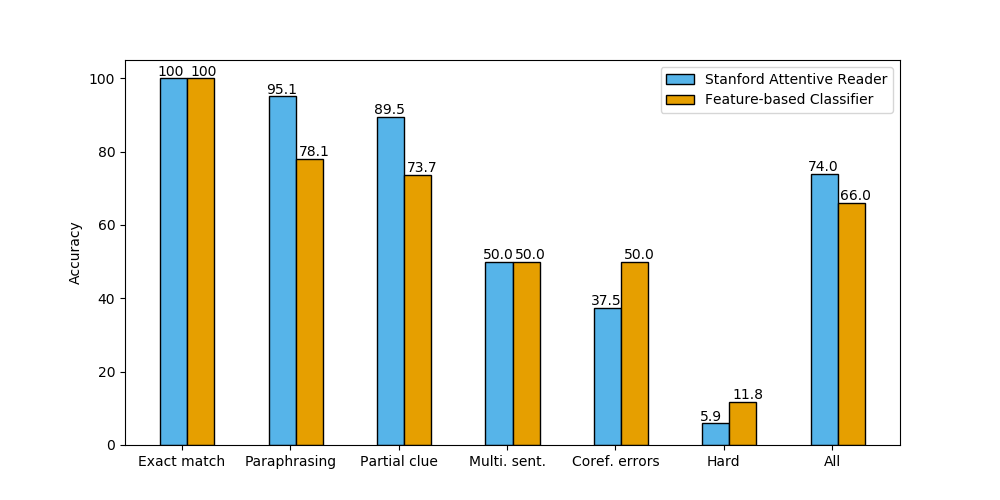
\includegraphics[scale=0.6]{img/cnn_analysis.png}
    \longcaption{The per-category performance of our two systems}{\label{fig:category-performance} The per-category performance of our two systems: the \sys{Stanford Attentive Reader} and the feature-based classifier, on the sampled 100 examples of the \sys{CNN} dataset.}
\end{figure}

% \begin{table}[h]
%    \centering
%     \begin{tabular}{@{} l  r @{\hspace*{0.25em}} r r @{\hspace*{0.25em}} r @{}}
%       \toprule
%      {Category} &  \multicolumn{2}{c}{{Classifier}} & \multicolumn{2}{c}{{Neural net}} \\
%     \midrule
%      Exact match & 13 & (100.0\%) & 13 & (100.0\%) \\
%      Paraphrasing &  32 & (78.1\%) & 39 & (95.1\%) \\
%      Partial clue & 14 & (73.7\%) &  17 & (89.5\%) \\
%      Multiple sentences &  1 & (50.0\%) & 1 & (50.0\%) \\
%     \midrule
%      Coreference errors &  4 & (50.0\%) & 3 & (37.5\%)\\
%      Ambiguous / hard &  2 & (11.8\%) & 1 & (5.9\%)  \\
%      \midrule
%      All & 66 & (66.0\%) & 74 & (74.0\%) \\
%     \bottomrule
%     \end{tabular}
%     \longcaption{The per-category performance of our two systems}{\label{tab:category-performance} The per-category performance of our two systems: the \sys{Stanford Attentive Reader} and the feature-based classifier, on the sampled 100 examples of the \sys{CNN} dataset.}
% \end{table}


Let's further take a closer look at the per-category performance of our neural network and feature-based classifier, based on the above categorization. As shown in Figure~\ref{fig:category-performance}, we have the following observations: (i)~The exact-match cases are quite simple and both systems get 100\% correct. (ii)~For the ambiguous\slash hard and entity-linking-error cases, meeting our expectations, both of the systems perform poorly. (iii)~The two systems mainly differ in the paraphrasing cases, and some of the ``partial clue'' cases. This clearly shows how neural networks are better capable of learning semantic matches involving paraphrasing or lexical variation between the two sentences. (iv)~We believe that the neural network model already achieves near-optimal performance on all the single-sentence and unambiguous cases.

To sum up, we find that neural networks are certainly more powerful at recognizing lexical matches and paraphrases compared to conventional feature-based models; while it is still unclear whether they also win out on the examples which require more complex textual reasoning as the current datasets are still quite limited in that respect.
